\documentclass[conference]{IEEEtran}
\usepackage{algorithmic}
\usepackage[pdftex]{graphicx}
\graphicspath{{imgs/}}
\DeclareGraphicsExtensions{.pdf,.jpeg,.png}

\begin{document}
\title{COSC 3P71 Final Project: \\ Chess Program with Game Tree Based AI}

\author{\IEEEauthorblockN{Sarah Childs}
	\IEEEauthorblockA{Brock University\\
		Student 5491018\\
		Email: sc15fv@brocku.ca}
	\and
	\IEEEauthorblockN{Matthew Grahlman}
	\IEEEauthorblockA{Brock University \\
		Student 5875695\\
		Email: mg15tm@brocku.ca}}

\maketitle

\section{Introduction}
This report will outline the decisions made as a team while designing, implementing, and testing our final project for COSC 3P71, which was to create the game of chess from scratch. The game follows all of the standard rules of chess, including castling, en passant and piece promotion. We decided to use the Java language to develop the project. We created a chess game which puts a player versus a computer player, with a difficulty that the player can set. The user is able to input their moves through the Java console. The computer player uses a game tree scheme that uses alpha-beta pruning in order to decide its move. The user is able to start a new game, or import a file with a custom board configuration which they can either customize or export from a previous game.

\subsection{Requirements}
The required features of this chess game were to respect the rules of chess, which include: the movement of pawns, rooks, knights, bishops, queens, and kings, castling, en passant, pawn promotion, check, checkmate, and stalemate. Additionally, the chess game had to use a game tree search scheme which incorporates alpha-beta pruning for the black team's AI. The game must also take into consideration a variety of user controlled parameters, which includes the depth of search. Another required feature was that the chess game must interact with a human player, where moves are given via board coordinates. At minumum, the program must output the board after each move as an ASCII table. A graphical user interface would have also been acceptable, however we decided to not implement one. Finally, the game must allow for any board configuration to be used by default, as well as the option to export the current configuration of the board at any given time.


\section{Game play}
\subsection{Reading the Console}
This chess game must be played through the Java console, thus it is very important that the user knows how read the ASCII chess board.
The topmost row of the chess board represents the columns numbers and the different valid entries the user can type into the console. Any piece in the column below these values are considered to be in that column, which will be important to remember while playing the game.
Additionally, the leftmost column of the chess board represents the row's letter values and the different valid entries that the user can type into the console. Similar to columns, any piece in this row is considered to be in that row, which will also be important to remember whilst playing the game.
The user can determine what team a given piece is on by looking at the first letter (in lowercase) of any non-empty space on the board. A "b" indicates that the piece belongs to the black team, while a "w" indicates that the piece belongs to the black team.
The user can also determine what type a given piece is by looking at the second letter(in uppercase) of any non-empty space on the board. A "P" indicates that the piece is a Pawn, "R" indicates that the piece is a Rook, "H" indicates that the piece is a Knight, "B" indicates that the piece is a bishop, "Q" indicates that the piece is a Queen, and a "K" indicates that the piece is a King.

\subsection{Console Input}
Upon being prompted for input the user will have three additional options. First, they can type "help" if they are unsure of what to do, how to play, or how a mechanic works. Additionally, they can type "export" to export the current configuration of the board to a file called "boardConfig", which is located in the "chessproject" folder, located in the "src" folder. Finally, the user may type "end" in order to end the game.

\begin{figure}[t!]
	\centering
	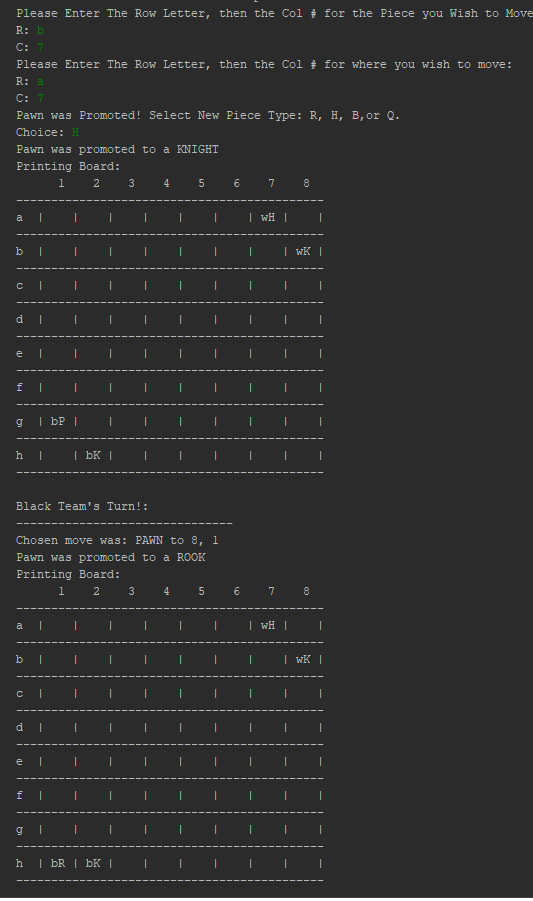
\includegraphics[clip,trim=0cm 0cm 3cm 0cm, width=3.5in, height=3in]{ss_promo}
	\caption{Screenshot of piece promotion for both sides.}
	\label{fig:piecepromo}
\end{figure}

When it is the player's turn, they will be first be prompted to select the piece they wish to move. The piece to move is selected by typing the that piece's row and column values. If the user selects a piece, but then decides they no longer want to move that piece, they may reselect the piece to move, refer to the "moveReselect" help code.

After selecting the piece to move, the user will be prompted for the row and column values for where they wish to move. It is important to note that to take an enemies piece, you must input the enemy piece's row and column values. For En Passant, the row and column values would be the empty space above (since you, as the player, are the white team) the enemies pawn. For Castling, the row and column values would be 2 spaces to the left or right of the King, where all other conditions for castling are met.

When one of the player's pawn's reach the opposite end of the board, that player's pawn will be promoted to a Rook, Knight, Bishop, or Queen. The user selects which piece type they wish to promote the move to and after doing so their turn will end. Refer to the "promotion" help code for additional information. Refer to Fig. \ref{fig:piecepromo} for an example input of piece promotion in game. 


\subsection{Help Codes}
In this game of chess there are instructions built into the game through help codes. To access these help codes the user can type "help" into the console at any time during their game. Once the user has entered this information a screen such a Fig. \ref{fig:helpcodes}, listing the available options. \\

\begin{figure}[t!]
	\centering
	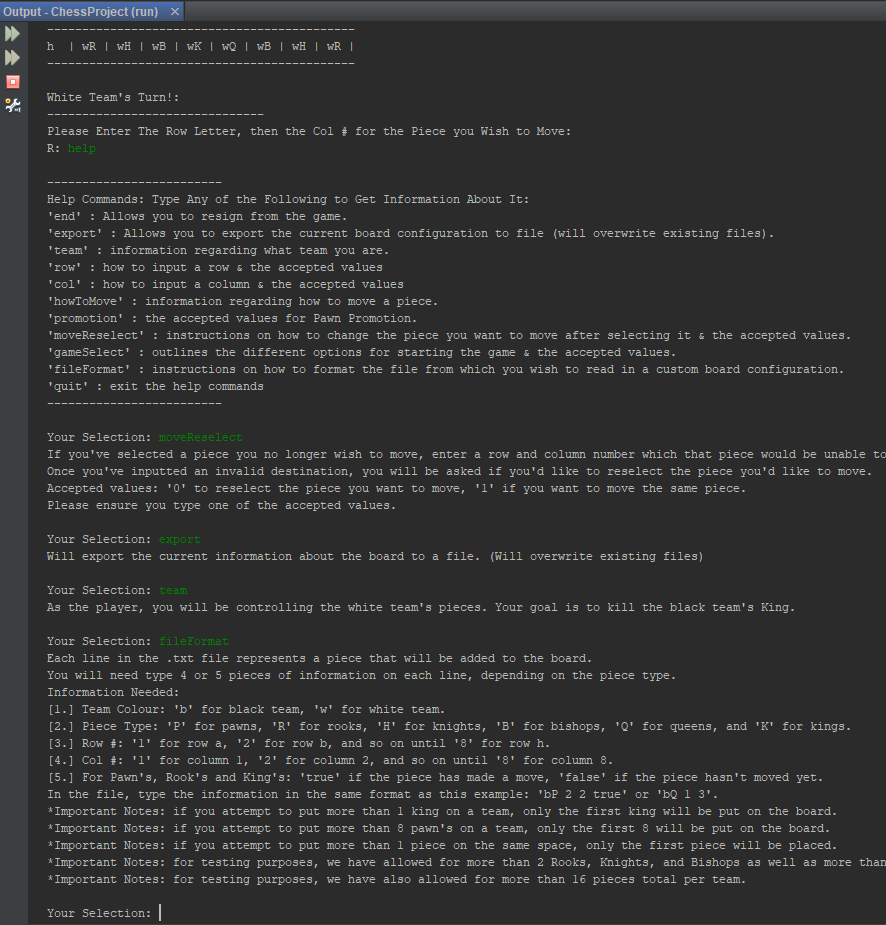
\includegraphics[clip,trim=1cm 3.5cm 0cm 3cm, width=3.5in, height=3in]{ss_helpcodes}
	\caption{Display of the help codes and their functionality.}
	\label{fig:helpcodes}
\end{figure}

The "team" help code gives the user information regarding which team they are controlling. In this chess game, the player will be controlling the white team's pieces, in their attempt to kill the black team's King.

The "row" help code instructs the user on how to input a row, as well as the accepted values. When it is the user's turn, they will be prompted for a row value for both the piece they are trying to move and the location they are trying to move that piece to. The accepted values for rows include; "a", "b", "c", "d", "e", "f", "g", and "h". If the user types in any other value, other than "help", "end" or "export", they will be prompted for the row value again. A user can determine what row a piece is in by looking at the leftmost column on the chessboard. For more information regarding reading the console and the chess board, please read "Reading the Console", above.

The "col" help code instructs the user on how to input a column, as well as the accepted values. When it is the user's turn, they will be promoted for a column value for both the piece they are trying to move and the location they are trying to move that piece to. The accepted values for columns include; "1", "2", "3", "4", "5", "6", "7", and "8". If the user types in any other value, other than "help", "end", or "export", they will be prompted for the column again. A user can determine what column a piece is in by looking at the topmost row on the chessboard. For more information regarding reading the console and the chessboard, please read "Reading the Console", above. 

The "howToMove" help code walks the user through the process of moving one of their pieces, which is done in two steps. First, the user will be prompted for both the row and column values for the piece in which they wish to move. For example, if the user wishes to move a Pawn in row b and in column 2, they would enter those values respectively when prompted. If the user selects a piece, but decides they no longer wish to move that piece, they may reselect the piece to move. Refer to the "moveReselect" help code. Secondly, the user will be prompted for the row and column values for where they wish to move the piece. Using the sample example, if we wish to move the Pawn to row c, column 3, we would type in those values respectively when prompted. It is important to note that if you wish to take an enemies piece, you must enter the coordinates of the enemy piece you wish to take, assuming the piece selected can in fact take that piece. For En Passant, the row and column values would be the empty space above (since you, as the player, are the white team) the enemies pawn. For Castling, the row and column values would be 2 spaces to the left or right of the King, where all other conditions for castling are met.

The "promotion" help code informs the user of the accepted values for pawn promotion. Pawn promotion will occur when one of the player's pawn's reaches the opposite end of the board. Upon this occurring, the player will be prompted to select which type of piece they would like to promote their pawn to. Pawn's are able to be promoted to: Rook's, Knight's, Bishop's, and Queen's. The accepted values for pawn promotion include: "R" for Rooks, "H" for Knights, "B" for Bishops, and "Q" for Queens. The user must type of one these accepted values into the console before being able to proceed playing the game.

The "moveReselect" help code walks the user through the process of reselecting the piece they wish to move. If the user changes their mind about which piece they would like to move, they may enter any row and column number that that piece would be unable to move to. Upon doing so, they will be asked if they would like to reselect the piece they are trying to move. The accepted values for this process include: "0" to reselect the piece to move and "1" to move the same piece they previously selected. The user must type of one these accepted values into the console before being able to proceed playing the game.

The "gameSelect" help code walks the user through their options upon starting the game, as well as the accepted values. When the game starts, the user will have two options: to start a new game or to load a custom board configuration from a file (for more information on this, refer to the "fileFormat" help code). The accepted values are: "0" to start a new game, with the default board configuration and "1" to load a custom board configuration from a .txt file. Starting a new game will immediately start the game. However, to load a custom board configuration the user must open the JFileChooser and navigate to the file they wish to read in. If the JFileChooser does not appear automatically, please wait several seconds, then press ALT and TAB and look for an open window named "Open". Navigate to this window and select the file. Upon doing so the game will start, failure to do so will result in a new game being started with the default board configuration. The user must type of one these accepted values into the console before being able to proceed playing the game.

The "fileFormat" help code walks the user through the process of setting up a .txt file from which they can load into the game as a custom board configuration. Each line in the .txt file represents a piece that will be added to the board. For each piece, you will need to include 4 or 5 pieces of information on each line, depending on the piece's type, which can be seen listed below:

\begin{enumerate}
	\item Team Colour: "b" for black team, "w" for white team.
	\item Piece Type: "P" for Pawns, "R" for Rooks, "H" for Knights, "B" for Bishops, "Q" for Queens, and "K" for Kings.
	\item Row as a number: "1" to place the piece in row a, "2" to place the piece in row b, and so on until "8" to place the piece in row h.
	\item Col as a number: "1" to place the piece in column 1, "2" to place the piece in 2, and so on until "8" to place the piece in column 8.
	\item If the Piece is a Pawn, Rook, or King you must also include: "true" if the piece has made a move or "false" if the piece has not yet made a move.
\end{enumerate}	

Important Notes regarding the "fileFormat" help code: attempting to put more than one King per team will result in only the first King being placed on the board. Each team must have a King, otherwise the program will crash since chess can not be played without Kings. Additionally, the user is limited to placing eight Pawn's per team on the board. Any additional Pawn's after the first eight will be ignored and not placed on the board. Next, attempting to place more than one piece on the same space will result in only the first piece being placed. For testing purposes, we have allowed for more than two Rook's, Knight's, Bishop's to be placed, as well as the opportunity to place more than one Queen. Additionally, we have also allowed for more than 16 pieces per team, again for testing purposes.\\

The "quit" help codes allows the user to exit from the help code commands.

The "end" help code allows the user to end the game at any time. This help code may be used outside of the help code commands.

The "export" help code allows the user to export the current board's configuration. This help code may be used outside of the help code commands. The resulting file is named "boardConfig", and can be found in the within the "chessproject/src" folder, which is located in the root of the submission.

	
\section{Back-end Design}
We chose to represent our pieces using two characters to ensure that there is no confusion with what piece the player is looking at at any given time. By representing the team using a lowercase letter and the piece type as an uppercase letter, we feel like we have achieved this.

The board is represented by an eight by eight 2D array of type Pieces, which is the abstract parent class used to represent any given piece.

The board is printed after each move and is done in two steps. The first step is setting every piece in the Board array to null. Then the pieces that have yet to be captured, which are stored in ArrayLists, on each team are added to the board at their current position.

We implemented piece movement by two different sets of values. First, we get the difference between the piece's row number and the row number for which the piece is attempting to move to. Then, we got the difference between the piece's column number, and the column number for which the piece is attempting to move to.

Pieces are able to move in vertical lines by taking the absolute value of the difference between the row values, where the difference between the column values is 0, and while also checking if there are pieces in the way of the piece making the move.

Pieces are able to move on diagonals when the absolute value of the difference between the row value and the column values are the same, and when there are no pieces in the way of the piece making the move.

Pieces are able to move in horizontal lines by taking the absolute value of the difference between the column values, where the difference between the row values is 0, and while also checking if there are pieces in the way of the piece making the move.

Knight's are able to move in L shapes by taking the absolute values of the difference between the row values and the column values, where the difference in row values is either 1 or 2, and where the difference between column values is 2 or 1, respectively. When these conditions are met, the Knight will move providing there isn't an ally piece at the location it is trying to move to.

For Pawns, Rooks, and Kings, we need to record whether or not they have made a move yet, for en passant, castling, and the pawn's ability to move two spaces on its first turn. This was achieved using a boolean variable, which was set to true when the piece makes a move. 

In the scenario in which there is a piece at the location we are attempting to move, we check if the piece is on the enemy team and if it is we make the move, assuming the pieces other conditions are met.

\subsection{Determination of States}
Chess has four primary states during a game: 
\begin{itemize}
	\item Play
	\item Check
	\item Checkmate
	\item Stalemate
\end{itemize}

When in play all moves are possible except those that would put the playing team's king in check; whereas when in Check only moves that will allow the king to be removed from check can be played. These moves consist of moving the king to a safe space, capturing the threat piece, or guarding the king with another piece. When none of those conditions can be met then the game is said to be in Checkmate, and it ends. In the case of a Stalemate, this occurs when no legal moves can be made by the player but they are not currently in check.

The state of the board was determined by looking at who had made the most recent move and considering what position they have placed their opponent in. Play was state as the default, if none of the other cases were true then the game was automatically in play. For Check, the board was evaluated by looking at the opponent's king and determining if any of the playing side's pieces could directly attack it. If any of the pieces were deemed a threat then the program would evaluate for Checkmate with specific criteria. If the Checked king is able to move to any space around him and be safe from the check then he is not Checkmated. If the king can not move safely, the program then considers if there are any ally pieces can capture the piece causing the check. Accordingly, if no piece can capture the threat, then it checks if any ally piece can guard the King from the threat. If none of these conditions can be met then the game is said to be in Checkmate.

To determine Stalemate the program considers if there is a threat of Check, if there is none then it can proceed to check if all pieces on the opponent's side can make a legal move. Should none of them be able to do so then the game is ended in a Stalemate, as the next player cannot make a move without checking/checkmating themselves.

These states are then used in the game loop to determine when to end the game, and on what terms the game ended with. They are also used in the evaluation of the board configurations for the AI opponent. 

\subsection{Artificial Intelligence}
As required by the assignment the AI opponent in our project uses the Minimax algorithm to decide which move it will take. This algorithm simulates the turns between each player given every possible move available to them. These actions are generated based on the board state that is passed through the recursive function, each node has to consider its own board configuration. This avoids issues that might arise on the playing board, but also allows for the proper evaluation given removal of pieces. 

As the algorithm simulates the turns, one function is trying to maximize the evaluation of the board (MAX), whereas the other attempts to minimize it (MIN); they are adversaries with the intent on winning. As mentioned in class, this algorithm assumes that the opponent will pick the lowest evaluation score, however if the opponent does not this can lead to the AI performing better than it would against MIN.

To allow for the best piece movement to be kept track of alongside the evaluation score that it produced, we introduced the AIAction class which contains the piece data, its destination position, and the evaluation score that was produced by the terminal or cutoff states. These AIAction objects were returned from the recursive calls and then updated in the case that the move produced a better result than the current best. This method of passing data was used to prevent any lose of information when recursively following the path to terminal case and popping back up, we wanted to make sure that the action information was kept, and used to update the current best value. 

The terminal case for the algorithm is determined using the current depth passed in through parameters, and the updated state of the board. If the depth of the tree has reached the designated ply depth then the tree will be cutoff prematurely to prevent further iterations. Otherwise, if the updated state of the board is Stalemate or a Checkmate then the search is terminated as that game is over. This ply depth allows the algorithm to look as many layers down in the tree until it reaches that depth limit, for our game this is restricted to between 2 and 6. Where 2 is considered an easy AI, and 6 is considered advanced, this is because the number of turns these AI can look at in advance to making a single move.

\subsection{Evaluation}
When considering the heuristic evaluation of the board configuration we decided to calculate multiple values and use those to influence the evaluation. As a human player does not only consider one or two points when determining their move, we thought that our AI should also consider more of what a human player would, as such, the equation seen in below was used to determine the value of each board configuration. \\

EVAL = \textit{(Current State value + (\# of Attackable Spaces for H/B) + (Summed weights of Capturable Pieces - Summed weights of Threatened pieces) + Center Influence) * Ratio of Black/White pieces} \\

Each portion of the evaluation will be explained below.
-What it is
- What its meant to do for AI
- How its calculated
-Why I designed it

\subsubsection{Current State}
The \textit{Current State value} is the value of which the current state of the board has associated with it. Play is considered a neutral state so it has no influence over the AI, whereas Checkmate has a very high value associated with it to encourage the AI to steer towards it. Check is similar, however its value is much less of Checkmates to reflect the relationship between the two states. Stalemate however, is represented as a negative value because traditionally it is considered to be draw. A draw is not inherently good or bad, however winning is the better option so that is reflected by the value of stalemate. 

This is meant to encourage the AI to move towards higher valued states, while also encouraging the MIN algorithm to aim for a draw if it has the opportunity. If these values were not included in the evaluation we can assume that the AI may still function properly, however it would not be as encouraged by Checks and Checkmates as it potentially could.

\subsubsection{Attackable Spaces}
The number of attackable spaces is calculated solely for the Bishop and Knight, and modifies the returned value based on their weight to prevent the value from taking over the equation. This portion of the evaluation is meant to favour piece development, an idea where the more spaces your stronger pieces can reach the better your odds of winning or controlling the board are. 

This is meant to influence the AI to move the stronger pieces to areas where they have more control over the board, rather than keeping them tucked away at the back. It is calculated by determining how many spaces in the piece's range of motion can they move to given the current board configuration. For example, at the default starting position a bishop cannot move any spaces, whereas the Knight can move to two. Yet if they were closer to the center then they both influence the "power" squares, and have a greater range of motion. 

This was added to the evaluation as mentioned to influence board configurations where pieces with higher values have greater ranges of motion on the board, giving the AI a stronger control. 

\subsubsection{Capturable \& Threatened Pieces}
These were summations of the weights for pieces that can be captured, and are threatened given the current board. These weights influence what boards have more potential to capture or protect stronger pieces. Capturable pieces are pieces on the opponent's side that are within range of at least one other piece, their weight is summed together with any other capturable pieces. Threatened pieces are those on the playing side that are within range of at least one of the opponent's pieces, their weight is then summed together as well with any other threatened pieces. 

This was designed to encourage the AI to look at itself, and how it's currently configured on the board and how it can protect itself through retreat, or capture of opponent pieces. As there is a small multiplier for the capturable sum, there is a stronger pull towards being able to capture pieces than to protect their own. 

This was calculated by checking each piece in the AI's team to see if they could move to a space with an opponent piece on it, or if an opponent piece could move to their position on the board. Each time either of those was true it added the weight of the threatened piece to the corresponding sum. 

\subsubsection{Center Influence}
Hi
\subsubsection{Ratio of Pieces}
you

\section{Known Bugs}
The following is a list of known bugs in the project and our potential solutions to fix them. These solutions were not implemented or tested due to time limits. 

\subsection{Rook Checkmate}
When using the Rook to checkmate the opponent it is possible for a checkmate to be triggered despite the King having escape routes, potential guards, and with the Rook in a capturable position. The cause of this bug is believed to be in the CheckMove function of the piece and how it calculates the spaces between its position and the destination. There was a potential solution implemented to allow for the ignoring of legality checks which may have led to the issue. Since this solution was implemented the bug has not been encountered, however it is very likely the issue lied elsewhere. 

\subsection{AI Move Coordinates}
This is not a bug, however it is a feature left over from testing that was not able to be completed in time. As it did not effect the gameplay we decided to leave it. When the AI outputs its chosen move coordinates the row value is displayed in numbers, rather than letters like the player's input requires. 

\section{Conclusion}
what we learned from this project? How we would better design our heuristics in the future?\\
\end{document}